\documentclass[11pt,letterpaper]{article}
\PassOptionsToPackage{hyphens}{url}
\usepackage[margin=.83in,top=.8in,bottom=.8in,headheight=15pt]{geometry}
\usepackage[T1]{fontenc}
\usepackage{lmodern,amsmath,amssymb,mathtools,bm,booktabs,array,graphicx,tikz}
\usetikzlibrary{arrows.meta,positioning,calc,decorations.pathreplacing,patterns}
\definecolor{ink}{HTML}{17344D}\definecolor{accent}{HTML}{087E8B}\definecolor{pale}{HTML}{EDF5F5}\definecolor{gold}{HTML}{AD6B19}
\providecommand{\dd}{\,\mathrm{d}}\providecommand{\R}{\mathbb{R}}
\providecommand{\E}{\mathbb{E}}\providecommand{\Var}{\operatorname{Var}}
\providecommand{\Cov}{\operatorname{Cov}}\providecommand{\diag}{\operatorname{diag}}
\providecommand{\norm}[1]{\left\lVert#1\right\rVert}
\providecommand{\abs}[1]{\left|#1\right|}
\usepackage{microtype,hyperref,fancyhdr,enumitem,amsthm,sectsty,needspace}
\allsectionsfont{\raggedright}
\hypersetup{colorlinks=true,linkcolor=ink,urlcolor=accent,pdfauthor={Zan Ahmad},pdftitle={Streamfunctions on a mapped chamber domain / Lecture notes}}
\setlength{\parindent}{0pt}\setlength{\parskip}{6pt}\linespread{1.07}
\setlist{itemsep=3pt,topsep=4pt,leftmargin=*}
\emergencystretch=2em\clubpenalty=10000\widowpenalty=10000
\pagestyle{fancy}\fancyhf{}\fancyhead[L]{\small Computational Cardiology}\fancyhead[R]{\small Lecture 8}
\fancyfoot[L]{\footnotesize Zan Ahmad}\fancyfoot[R]{\footnotesize\thepage}\renewcommand{\headrulewidth}{.3pt}
\newtheorem{proposition}{Proposition}\newtheorem{theorem}{Theorem}\newtheorem{lemma}{Lemma}
\theoremstyle{definition}\newtheorem{definition}{Definition}\newtheorem{example}{Example}
\numberwithin{equation}{section}
\begin{document}
{\small\scshape Computational Cardiology\hfill Lecture 8}\par\medskip
{\raggedright\hyphenpenalty=10000\exhyphenpenalty=10000\LARGE\bfseries\color{ink} Streamfunctions on a mapped chamber domain\par}\medskip
{\small Lecture notes}\par\bigskip
A streamfunction constructs an incompressible planar velocity field without solving momentum balance. On a widening domain, the coordinate transformation must be included in every derivative. This construction also supplies a precise nonuniqueness example: different interior motions can have identical wall conditions and port flow.

\section{Prescribed kinematics and the unresolved momentum balance}
\hypertarget{note-prescribed-kinematics-and-the-unresolved-momentum-balance}{}\label{note:prescribed-kinematics-and-the-unresolved-momentum-balance}
{\small \href{slides.html\#frame=incompressibility-as-a-kinematic-constraint\&step=1}{Slides for this section} \quad \href{../modules/cfd/index.html}{Conservation, viscous flow and transport}}\par
This lesson uses a deliberately transparent atrial-inspired fixture: a fixed widening two-dimensional channel with one inlet and one outlet, extruded through a constant depth. It is not a reconstructed atrium, does not include four pulmonary veins or a moving mitral valve, and contains no patient data. Its prescribed velocity lets us know the exact reference while practicing diagnostics that a more complete study would also need.

The motivating question is whether conservation and a visually plausible interior flow are enough. We construct two internal velocity fields with identical geometry and port flow, then compare their patterns. Their differences show that a single integrated observable cannot uniquely determine the full field. A useful report must therefore name both the observable that is checked and the unresolved features that it cannot constrain.

The distinction is mathematical: $\nabla\cdot u=0$ is one scalar constraint on two velocity components, whereas the viscous momentum equations impose additional differential constraints involving pressure and forcing. Specifying a divergence-free field solves the first requirement only. A plausible geometry cannot supply the missing pressure equation.
\section{A widening domain and its volume}
\hypertarget{note-a-widening-domain-and-its-volume}{}\label{note:a-widening-domain-and-its-volume}
{\small \href{slides.html\#frame=the-mapped-chamber\&step=1}{Slides for this section} \quad \href{../modules/cfd/index.html}{Conservation, viscous flow and transport}}\par
The chamber length is L=0.06 m. Its lower wall is y=0 and its upper wall has height H(x)=H0[1+b sin\ensuremath{^{2}}(\ensuremath{\pi}x/L)], with H0=0.01 m and b=1.5. The inlet and outlet gaps are 10 mm and the maximum height is 25 mm. The out-of-plane width is W=0.02 m. All of these values are synthetic choices. A uniform computational coordinate \ensuremath{\eta} runs from zero to one and maps to physical height y=\ensuremath{\eta}H(x).

The exact volume of the extruded chamber is W H0 L(1+b/2), because the average of sin\ensuremath{^{2}} over the length is one half. It is 21 mL for these values. Prescribe flow per width q=2\ensuremath{\times}10\ensuremath{^{-4}} m\ensuremath{^{2}}/s, giving total flow Q=Wq=4 mL/s. Volume divided by flow is then 5.25 s. This is a bulk turnover scale: it does not say that every particle leaves after 5.25 s or that an appendage has been washed out.

Input sensitivity is a separate experiment from mesh refinement. Multiplying q by 0.8 or 1.2 leaves geometry unchanged but changes the prescribed flow to 3.2 or 4.8 mL/s. The bulk scale becomes 6.5625 or 4.375 s. These differences are exact consequences of the input choice. Reducing a derivative-discretization error cannot resolve uncertainty about which boundary waveform or amplitude is appropriate for a real subject.

\[
H(x)=H_0[1+b\sin^2(\pi x/L)],\qquad y=\eta H(x)
\]
0\ensuremath{\le}x\ensuremath{\le}L and 0\ensuremath{\le}\ensuremath{\eta}\ensuremath{\le}1; H0=10 mm, L=60 mm and b=1.5.

\[
V=WH_0L(1+b/2),\qquad Q=Wq,\qquad T_{\rm bulk}=V/Q
\]
V=21 mL, Q=4 mL/s and T\_bulk=5.25 s for the baseline.

The map $(x,\eta)\mapsto(x,\eta H(x))$ has Jacobian determinant $H(x)>0$. Therefore
\[
 V=W\int_0^L\int_0^1H(x)\,\mathrm d\eta\,\mathrm dx
   =WH_0L(1+b/2).
\]
At fixed geometry, $T_{\rm bulk}=V/Q$ satisfies $\delta T_{\rm bulk}/T_{\rm bulk}=-\delta Q/Q$ to first order. It is an integral volume-to-flux ratio, not a particle residence-time distribution.

\paragraph{Calculation.} Compute the baseline volume and the effect of a 20\% higher prescribed flow.

Volume is 0.02\ensuremath{\times}0.01\ensuremath{\times}0.06\ensuremath{\times}1.75=2.1\ensuremath{\times}10\ensuremath{^{-5}} m\ensuremath{^{3}}=21 mL.

Baseline flow is 0.02\ensuremath{\times}2\ensuremath{\times}10\ensuremath{^{-4}}=4\ensuremath{\times}10\ensuremath{^{-6}} m\ensuremath{^{3}}/s=4 mL/s.

Increasing flow by 20\% gives 4.8 mL/s and 21/4.8=4.375 s.

The input perturbation changes the bulk scale by an exact inverse relation, independently of mesh error.
\section{Streamfunction construction in mapped coordinates}
\hypertarget{note-streamfunction-construction-in-mapped-coordinates}{}\label{note:streamfunction-construction-in-mapped-coordinates}
{\small \href{slides.html\#frame=a-through-flow-streamfunction\&step=1}{Slides for this section} \quad \href{../modules/cfd/index.html}{Conservation, viscous flow and transport}}\par
In two dimensions a streamfunction \ensuremath{\psi} defines u=\ensuremath{\partial}\ensuremath{\psi}/\ensuremath{\partial}y and v=\ensuremath{-}\ensuremath{\partial}\ensuremath{\psi}/\ensuremath{\partial}x. Equal mixed derivatives cancel in the divergence, giving a continuous divergence-free field when \ensuremath{\psi} is smooth. The difference in \ensuremath{\psi} between two points on a cross-section equals flow per width across it. These facts make streamfunctions useful verification fixtures; they do not establish the momentum equation.

Our base streamfunction is q times f(\ensuremath{\eta}), where f=3\ensuremath{\eta}\ensuremath{^{2}}\ensuremath{-}2\ensuremath{\eta}\ensuremath{^{3}}. It gives a parabolic port profile with zero velocity at the side walls. Add \ensuremath{\alpha}q sin\ensuremath{^{2}}(\ensuremath{\pi}x/L) g(\ensuremath{\eta}), where g=\ensuremath{\eta}\ensuremath{^{2}}(1\ensuremath{-}\ensuremath{\eta})\ensuremath{^{2}}. This added term and its needed wall derivatives vanish on the side walls and at the ports. Changing \ensuremath{\alpha} therefore alters the interior while preserving the same port flow and no-slip side-wall values. The figure contrasts \ensuremath{\alpha}=0 with \ensuremath{\alpha}=24, which includes internal reverse flow.

The mapped-coordinate derivatives must account for the changing H. If subscripts x and \ensuremath{\eta} denote derivatives at fixed computational coordinates, then u=\ensuremath{\psi}\ensuremath{\eta}/H and v=\ensuremath{-}\ensuremath{\psi}x+\ensuremath{\eta}H\ensuremath{^{\prime}}\ensuremath{\psi}\ensuremath{\eta}/H. Omitting the second term in v would differentiate at the wrong fixed coordinate. Even the correctly constructed field is only kinematic. We have supplied neither a pressure satisfying momentum balance nor a compatible viscous force, acceleration or forcing; incompressibility and no-slip do not guarantee those equations.

\[
\psi=q\{3\eta^2-2\eta^3+\alpha\sin^2(\pi x/L)\eta^2(1-\eta)^2\}
\]
\ensuremath{\psi} and q have m\ensuremath{^{2}}/s; \ensuremath{\alpha} is a dimensionless prescribed shape parameter.

\[
u=\psi_\eta/H,\qquad v=-\psi_x+\eta H^\prime\psi_\eta/H
\]
\ensuremath{\psi}x is differentiated at fixed \ensuremath{\eta}; the second term converts to a derivative at fixed y.

Since $\eta=y/H(x)$,
\[
 \left.\partial_x\right|_y=\left.\partial_x\right|_\eta-
 \frac{\eta H^{\prime}}H\partial_\eta,
 \qquad \partial_y=\frac1H\partial_\eta.
\]
Applying these identities to $u=\psi_y$ and $v=-\psi_x|_y$ yields the physical velocities in the companion. The base function $f(\eta)=3\eta^2-2\eta^3$ has $f(0)=0$, $f(1)=1$ and $f^{\prime}(0)=f^{\prime}(1)=0$. The perturbation $g(\eta)=\eta^2(1-\eta)^2$ and its first derivative vanish at both walls. Thus changing $\alpha$ preserves the port flux and the no-slip side-wall values.
\begin{center}\begin{minipage}{.98\linewidth}\centering
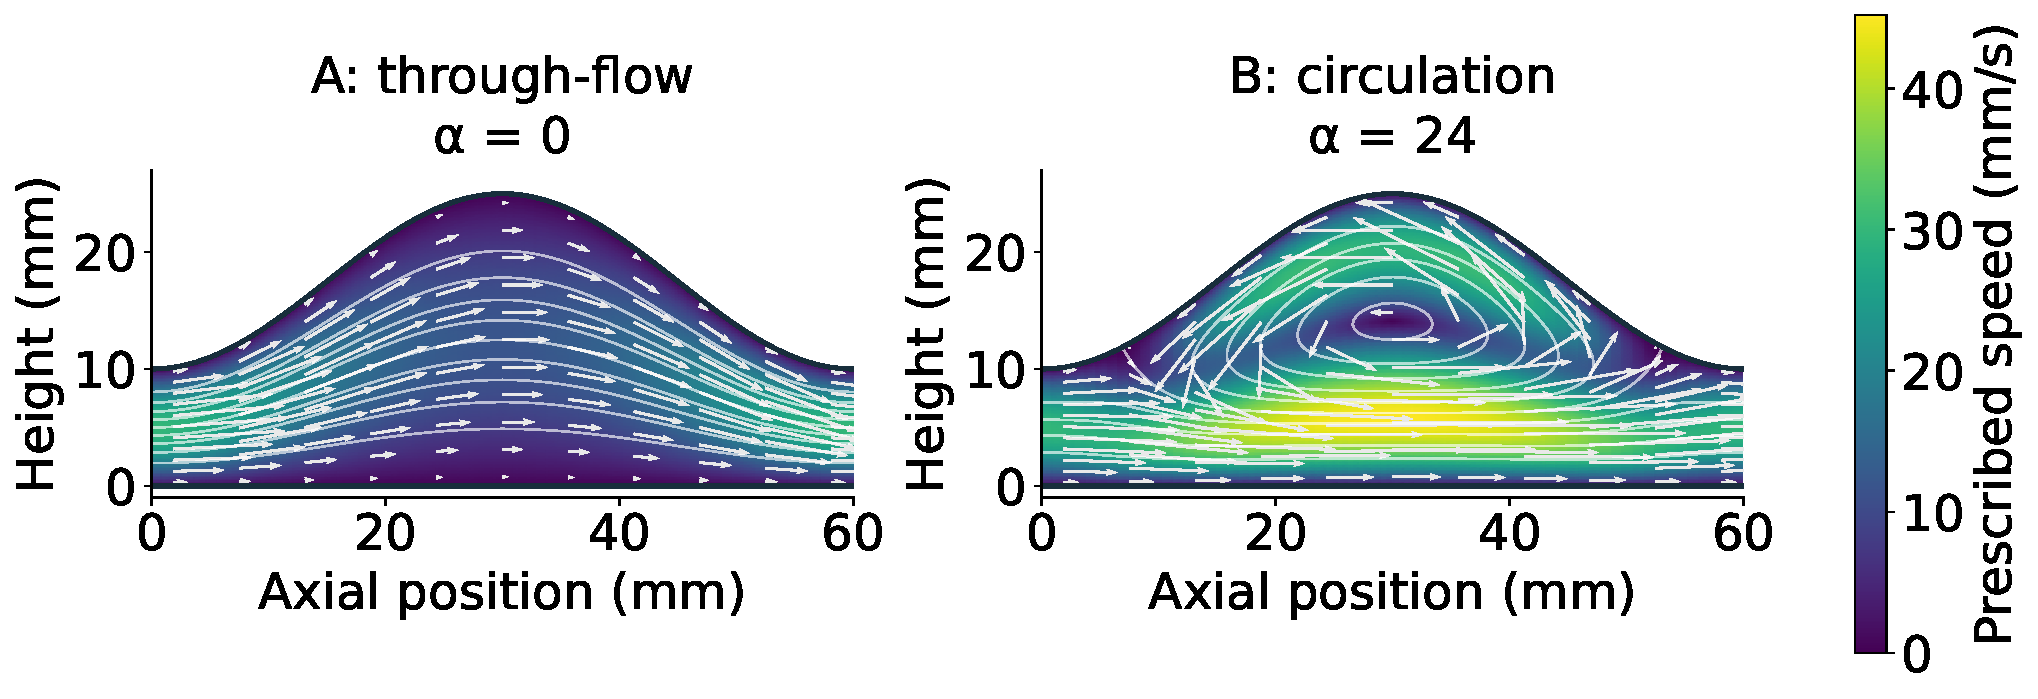
\includegraphics[width=.96\linewidth,height=.57\textheight,keepaspectratio]{synthetic-chamber.pdf}\par\smallskip
{\small Original fixed synthetic chamber: 60 mm long, 10--25 mm high and 20 mm deep. Both fields have 4 mL/s port flow and 21 mL volume. Velocity is prescribed, with no momentum solve.}
\end{minipage}\end{center}
\section{Cell fluxes and derivative reconstruction}
\hypertarget{note-cell-fluxes-and-derivative-reconstruction}{}\label{note:cell-fluxes-and-derivative-reconstruction}
{\small \href{slides.html\#frame=a-closed-cell-flux-identity\&step=1}{Slides for this section} \quad \href{../modules/cfd/index.html}{Conservation, viscous flow and transport}}\par
For each mapped cell, integrate velocity normal to each edge using the streamfunction difference between its endpoints. The four oriented edge differences cancel exactly because each corner appears once with each sign. The supplied face-flux diagnostic therefore closes to roundoff. This is a strong check on the shared-face implementation, but it is also built into the streamfunction construction. It should not be confused with an independent test of every sampled velocity component.

A second calculation reconstructs u and v from numerical derivatives of \ensuremath{\psi} on 16, 32, 64 and 128 intervals per computational coordinate. Comparing those values with the analytic velocities gives RMS errors that approach second order; the last observed order is approximately 1.995 in the supplied calculation. Here refinement measures a derivative reconstruction, not convergence of a Navier--Stokes solver. The exact reference and the operation being tested are explicitly identified.

The reusable velocity\_diagnostics function accepts sampled X, Y, u and v arrays on the documented mapped structured grid. It checks the coordinate layout, computes velocity-derived divergence, and integrates oriented inlet, outlet and side-wall fluxes. It can audit an imported field represented on that grid without using \ensuremath{\psi}. A deliberately injected upward leak produces a detectable 1.2 mL/s net outward flow. General unstructured meshes need their own geometry-aware face integration; passing this array interface does not establish a valid interpolation from another mesh.

\[
\sum_{e\in\partial K}F_e=0,\qquad \nabla\!\cdot\mathbf u=\left.\partial_xu\right|_\eta-\frac{\eta H^\prime}{H}\partial_\eta u+\frac1H\partial_\eta v
\]
The first is an integrated cell account; the second has units 1/s and includes derivative approximation error.

Orient a cell boundary counterclockwise. With $u=(\psi_y,-\psi_x)$, outward flux along an edge is $\mathrm d\psi$ along that orientation. Consequently,
\[
 \oint_{\partial K}u\cdot n\,\mathrm ds=\oint_{\partial K}\mathrm d\psi=0.
\]
The discrete edge differences telescope around the corners. By contrast, velocity-derived divergence uses separately approximated derivatives and can have a nonzero discretization residual.
\begin{center}\begin{minipage}{.98\linewidth}\centering
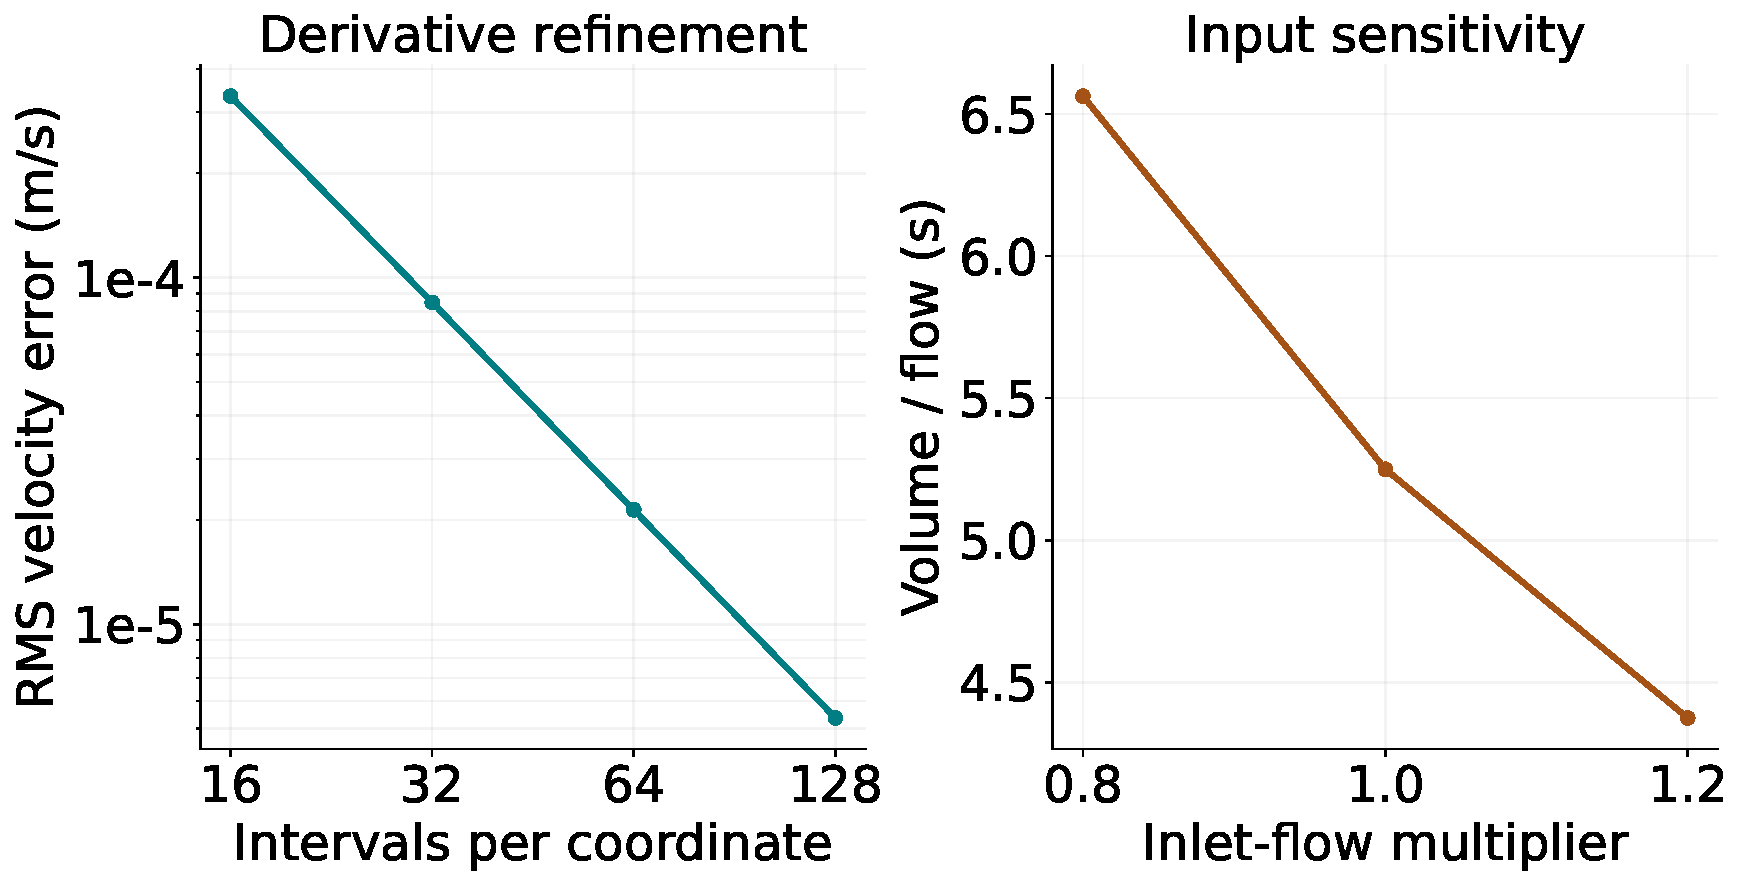
\includegraphics[width=.96\linewidth,height=.57\textheight,keepaspectratio]{chamber-verification.pdf}\par\smallskip
{\small Left: error of derivative reconstruction against an exact kinematic field. Right: exact bulk volume/flow sensitivity to prescribed inlet amplitude. Neither panel provides physiological validation.}
\end{minipage}\end{center}
\section{Integrated observations and interior nonuniqueness}
\hypertarget{note-integrated-observations-and-interior-nonuniqueness}{}\label{note:integrated-observations-and-interior-nonuniqueness}
{\small \href{slides.html\#frame=an-interior-perturbation\&step=1}{Slides for this section} \quad \href{../modules/cfd/index.html}{Conservation, viscous flow and transport}}\par
A real atrial CFD study would need a defensible three-dimensional geometry, a stated fluid model, pressure and velocity boundary conditions, and wall-motion data or an explicit fixed-wall approximation. It would solve the relevant momentum and mass equations with an independently checked numerical method. Iterative residuals, mesh and time refinement, boundary balances and limiting benchmarks would address different implementation and calculation errors. The current fixture does not supply those missing equations or solver evidence.

Validation would then compare relevant observables with independent physical measurements, including their uncertainties and acquisition conditions. A bulk flow measurement can test an integrated quantity, while a spatial velocity measurement can constrain interior motion. Reusing the same data to tune parameters and to claim independent validation weakens the evidence. A successful comparison must be tied to the intended application and tested regime rather than described as proof of universal correctness.

Divergence, mass and momentum residuals quantify different equations. A momentum residual requires terms such as acceleration, pressure gradient and viscous stress, none of which is fully specified by the present diagnostic interface. The function therefore reports momentum as not assessed. A small net boundary imbalance can also coexist with large local divergence that cancels over the domain, so inspect both quantities and their refinement rather than selecting whichever one looks smallest.

Let $\psi_0$ be the through-flow and $\chi$ the perturbation that vanishes at the ports. Then the family $\psi_\alpha=\psi_0+\alpha\chi$ has the same flux functional $\mathcal Q(\psi_\alpha)=q$ for every $\alpha$, while its velocity changes by $\alpha(\chi_y,-\chi_x)$. The integrated observable has a nontrivial nullspace. Measuring $Q$ alone cannot identify that interior component.

Here $\mathcal Q(\psi)=\psi(x,H(x))-\psi(x,0)$ is flux per unit width; total flow is $Q=W\mathcal Q(\psi)$.
\section{Sensitivity of a bulk turnover scale}
\hypertarget{note-sensitivity-of-a-bulk-turnover-scale}{}\label{note:sensitivity-of-a-bulk-turnover-scale}
{\small \href{slides.html\#frame=a-bulk-turnover-scale\&step=1}{Slides for this section} \quad \href{../modules/cfd/index.html}{Conservation, viscous flow and transport}}\par


For the synthetic values, $V=21$ mL and $Q=4$ mL/s give $T_{\rm bulk}=5.25$ s. The two perturbed flows $0.8Q$ and $1.2Q$ produce $6.5625$ and $4.375$ s, respectively. These are exact input sensitivities. They remain even if the derivative reconstruction error is driven to zero by refinement. A residence-time claim would additionally require trajectories, mixing assumptions and an explicitly defined exit event.
\bigskip
\section*{Exercises}
\par\noindent\begin{minipage}{\linewidth}
\subsection*{E1. Geometry and boundary sensitivity}
A synthetic widening chamber has L=\allowbreak{}0.05 m, H0=\allowbreak{}0.008 m, b=\allowbreak{}2 and W=\allowbreak{}0.025 m. Prescribe q=\allowbreak{}1.6$\times$10$^-$$^4$ m$^2$/s.

\textbf{a} Compute volume, total flow and V/Q.

\end{minipage}\par\medskip
\textbf{b} Reduce q by 25\% with geometry fixed. Compute the new bulk scale.

\textbf{c} Can mesh refinement decide which prescribed q is physically correct?

\par\noindent\begin{minipage}{\linewidth}
\subsection*{E2. Conservation does not supply momentum}
Two smooth chamber fields satisfy no-slip side walls, zero divergence and the same 4 mL/s inlet and outlet flows.

\textbf{a} What can be concluded from these facts?

\end{minipage}\par\medskip
\textbf{b} What additional evidence is required before claiming a Navier--Stokes solution?

\textbf{c} Name one independent measurement that could distinguish the interior fields.

\par\noindent\begin{minipage}{\linewidth}
\subsection*{E3. Read a derivative refinement and a leak}
On 20, 40 and 80 intervals, RMS velocity errors are 0.0012, 0.0003 and 0.000075 m/s. Separately, a sampled field has 5.0 mL/s inflow, 4.6 mL/s outflow and 0.1 mL/s outward side-wall flux.

\textbf{a} Compute the two observed orders and identify what is verified.

\end{minipage}\par\medskip
\textbf{b} Compute the net outward boundary flux. Is it compatible with a fixed incompressible no-source chamber?

\textbf{c} If net flux were zero, would local divergence necessarily be small?

\par\noindent\begin{minipage}{\linewidth}
\subsection*{E4. Draft a defensible report claim}
A group writes: ``Our atrial CFD is validated because its mass error is zero, and a finer mesh barely changes V/Q.''

\textbf{a} Identify three unsupported implications.

\end{minipage}\par\medskip
\textbf{b} Rewrite the claim for the present fixture.

\textbf{c} List two next evidence categories for a real atrial application.

\section*{References}
\noindent\begin{minipage}{\linewidth}
Zan Ahmad, Advanced Topics in Computational Cardiology syllabus, Fall 2024. PDF pages 1--2.

\end{minipage}\par\medskip
\noindent\begin{minipage}{\linewidth}
NASA NPARC Alliance, Overview of CFD Verification and Validation. Introduction and Use of CFD Results.

\url{https://www.grc.nasa.gov/www/wind/valid/tutorial/overview.html}
\end{minipage}\par\medskip
\noindent\begin{minipage}{\linewidth}
NASA NPARC Alliance, Validation Assessment. Validation; Requirements for Experimental Data.

\url{https://www.grc.nasa.gov/www/wind/valid/tutorial/valassess.html}
\end{minipage}\par\medskip
\end{document}
